\chapter{Diseño}

Al ser este un sistema \acrshort{RI} el diseño ha de girar en torno a los datos, por ello comencé explorando diversas alternativas para utilizar como fuente de datos. 

Como punto inicial para la extracción de los datos de los autores de la \acrshort{ETSIIT} partí del Ranking UGRinvestiga \cite{Ranking_UGRInvestiga}. En este se lista a todos los autores de la facultad junto con sus citas e índice h total y los últimos 5 años.

Sin embargo no hay modo de obtener datos de los artículos concretos por lo que barajé múltiples bases de datos bibliográficas, además de las ya comentadas en la sección \nameref{subsec:sistemasRI} también exploré \href{https://www.researchgate.net/}{Research Gate}.

Los resultados de mi análisis fueron los siguientes: 
\begin{itemize}
	
	\item Google Scholar y Research Gate parecen tener bastantes datos en comparación a otras opciones, sin embargo no ofrecen una \acrshort{API} por lo que la extracción de datos solo se podría llevar a cabo mediante \textit{\gls{webscraping}} \glsrefentry{webscraping}. Lo cual no es un proceso sencillo ya que muchas de estas web contienen mecanismos de detección de bots como los CAPTCHAs \cite{scrapping_GS} y además es un método muy sensible al cambio, en caso de que produzca alguna modificación en la web en cuestión es probable que toque reescribir el método de extracción de datos.
	\item \acrshort{WoS} y Scopus sí disponen de una \acrshort{API}, tras realizar algunas pruebas y leer opiniones sobre ambas me decanté por utilizar Scopus como fuente de datos ya que su \acrshort{API} me resultó más cómoda de utilizar y encontré datos fácilmente de algunos autores de la \acrshort{ETSIIT} (cosa que me costó bastante más en \acrshort{WoS}).
\end{itemize}

\section{Modelo de datos}

Siguiendo el modelo de Scopus decidí separar la búsqueda de autores y la de artículos ya que son dos tipos de datos muy diferenciados e intuitivamente se comprende que un sistema de \acrshort{RI} funcionará mejor si los datos son homogéneos.

Por tanto mi modelo de datos está constituido por 2 entidades distintas pero relacionadas: Autores (\textit{Author}) y Artículos (\textit{Abstract}). 

En las siguientes secciones se describen brevemente ambas entidades.


\subsection{\textit{Author}}

Esta entidad es resultado de la combinación de la información disponible en el Ranking UGRinvestiga \cite{Ranking_UGRInvestiga} y en Scopus, por eso podemos ver en el siguiente diagrama con el prefijo \texttt{ugr} las medidas de dicho ranking y con el de \texttt{scopus} los de la plataforma homónima. 

Respecto a los atributos que finalizan en \texttt{5} estos hacen referencia a los valores de dichas medidas de los últimos cinco años mientras que este sufijo no aparece las medidas son totales.

\begin{figure}[ht]
	
	\centering
	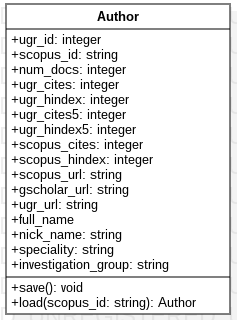
\includegraphics[width=0.4\linewidth]{imagenes/Author}
	\caption{Clase \textit{Author}}
\end{figure}

\newpage

\subsection{\textit{Abstract}}

La entidad \textit{Abstract} corresponde casi directamente con los datos obtenidos a través de la \acrshort{API} de Scopus, a excepción de:
\begin{itemize}
	\item Las referencias han sido limitadas a citas internas, es decir entre los artículos que están disponibles en la colección, con la idea de usar esta información en el proceso de búsqueda.
	\item Los autores, que únicamente aparecían listados con su \texttt{scopus\_id}, han sido enriquecidos con el nombre de los mismos así como el \texttt{ugr\_id} en caso de estar disponible este último (este identificador estará disponible si el autor es alguno de los que forman parte de la colección de autores).
\end{itemize}

\begin{figure}[h]
	
	\centering
	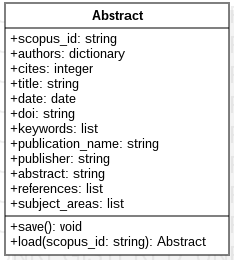
\includegraphics[width=0.4\linewidth]{imagenes/Abstract}
	\caption{Clase \textit{Abstract}}
\end{figure}

\newpage

\section{Arquitectura del sistema}

La arquitectura final del sistema es la de una aplicación web distribuida:
\begin{itemize}
	\item Un \textbf{cliente web} que se ejecuta en el navegador y constituye la interfaz de usuario, este se encarga de recoger las consultas, enviarlas al servidor de \acrfull{ES} y mostrar los resultados de las mismas sirviéndose de tecnologías como \textit{Searchkit}, \textit{ReactJS} o \textit{MaterialUI}. 
	
	\item Un \textbf{servidor Elastic} donde se ejecuta \acrshort{ES} y el cual contiene los índices de autores y \textit{abstracts} así como los datos indexados para la búsqueda (que no son todos los listados en el modelo de datos previamente).
	
	\item Un \textbf{servidor de monitorización} del servidor Elastic utilizando el proyecto de software libre Cerebro. Este permite monitorizar en tiempo real diversas medidas del servidor como la carga, espacio utilizado o estado además de múltiples funciones como un cliente REST que permite la consulta a bajo nivel sobre \acrshort{ES} muy utilizado para depuración o durante el desarrollo para hacer pequeñas pruebas.
	
	\item Un \textbf{servidor de aplicación} que utiliza \textit{Flask} para montar algunos microservicios auxiliares que permiten recuperar el resto del modelo de datos que no se encuentra indexado así como aportar algunas estructuras de datos precalculadas para facilitar la búsqueda.
	
	\item Un \textbf{servidor mongo} que lleva una \acrshort{BD} \textit{MongoDB} la cual contiene la totalidad de los datos de ambas colecciones y sirve como fuente de datos para el servidor de aplicación.
	
\end{itemize}

\begin{figure}[ht]
	
	\centering
	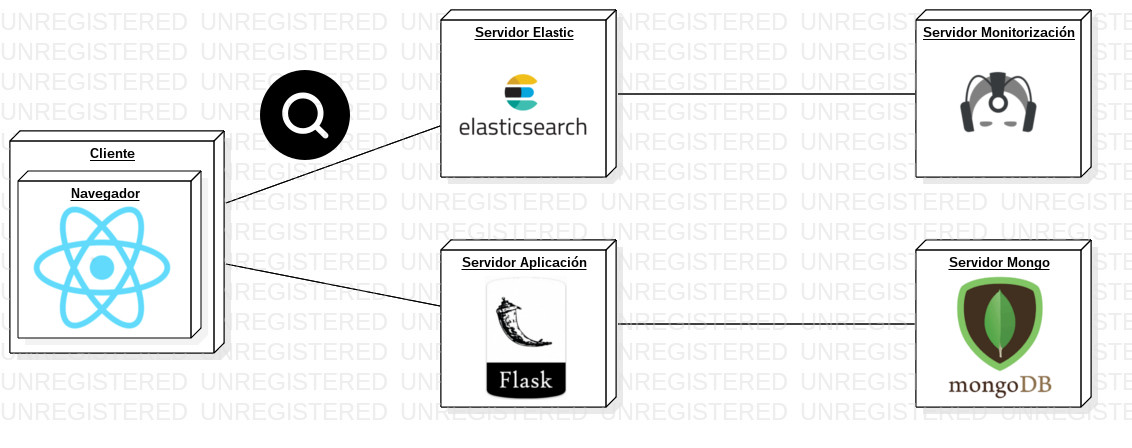
\includegraphics[width=\linewidth]{imagenes/achitecture}
	\caption{Diagrama de arquitectura final con las principales tecnologías usadas en cada nodo}
\end{figure}